\documentclass{beamer}

\mode<presentation> {
  \usetheme{Darmstadt} 
  \setbeamercovered{transparent}
}

\usepackage[french]{babel}
\usepackage[utf8]{inputenc}

\usepackage{times}
\usepackage[T1]{fontenc}
\usepackage{graphicx}

\title[Learning to tag]{Présentation de l'article \emph{Learning to tag} \\
    (Lei Wuk, Linjun Yang, Nenghai Yu, Xian-Sheng Hua, 2009)}

\subtitle {UE APAS M2 IAD}

\author[Decock, Ristic] % (facultatif, à utiliser seulement avec plusieurs auteurs)
{Jérémie~\bsc{Decock} \and Daniel~\bsc{Ristic}}
% - Composez les noms dans l'ordre dans lequel ils apparaîtrons dans l'article
% - Utilisez la commande \inst{?} uniquement si les auteurs ont des affiliations
%   différentes.

\institute[Universités Pierre et Marie Curie]
{
  %\inst{1}%
  Master d'Informatique\\
  Université Pierre et Marie Curie
}
% - Utilisez la commande \inst uniquement s'il y a plusieurs affectations

\date[]
{21 octobre 2009}

\subject{Rapport sur l'article "Learning to tag" (WWW 2009-361)}


% Si vous avez un fichier nommé "université-logo-nomfichier.xxx", où xxx
% est un format graphique accepté par latex ou pdflatex (comme par exemple .png),
% alors vous pouvez insérer votre logo ainsi :

% \pgfdeclareimage[height=0.5cm]{le-logo}{université-logo-nomfichier}
% \logo{\pgfuseimage{le-logo}}



% À supprimer si vous ne voulez pas que la table des matières apparaisse
% au début de chaque sous-section :

\AtBeginSection[] {
  \begin{frame}<beamer>{Plan}
    \tableofcontents[currentsection,currentsubsection]
  \end{frame}
}

% Si vous souhaitez recouvrir vos transparents un à un,
% utilisez la commande suivante (pour plus d'info, voir la page 74 du manuel
% d'utilisation de Beamer (version 3.06) par Till Tantau) :

%\beamerdefaultoverlayspecification{<+->}


\begin{document}

\begin{frame}
  \titlepage
\end{frame}

\begin{frame}{Plan}
  \tableofcontents
  % Vous pouvez, si vous le souhaiter ajouter l'option [pausesections]
\end{frame}


% Structurer l'entretien est une tâche difficile et la structure suivante
% pourrait ne pas convenir. Voici quelques règles à appliquer pour cet
% exemple ci :

% - Avoir exactement deux ou trois sections (autre que la table des matières).
% - Tout au plus trois sous-sections par section
% - Parlez approximativement entre 30 secondes et 2 minutes par transparent. Il
%   devrait donc y avoir entre 15 et 30 transparents, tous ayant été commentés.

% - Le public d'une conférence connaîtra probablement peu de chose sur le sujet
%   que vous serez en train de traiter. Donc, *simplifiez* !
% - Dans un exposé de 20 minutes, garder à l'esprit les idées principales est largement
%   suffisant pour votre assistance. Laissez tomber certains détails, même s'ils vous
%   semblent nécessaires.
% - Si vous omettez un détail qui est vital pour une preuve/mise en oeuvre,
%   dites le simplement une fois. Ce sera suffisant pour tout le monde.

% 1 %%%%%%%%%%%%%%%%%%%%%%%%%%%%%%%%%%%%%%%%%%%

\section{Le problème}

\begin{frame}{Pourquoi étiqueter ?}

	On souhaite pouvoir faire une recherche par mots clés sur des images.
	\begin{itemize}
        \item Une façon d'y arriver~: ajouter des tags
        \item Ne peut pas se faire automatiquement
	\end{itemize}

	Sur des sites comme \emph{Flickr}
	\begin{itemize}
        \item Énormément d'images (9 milliards en 2009)
        \item Fait par les utilisateurs (social tagging)
	\end{itemize}

\end{frame}

\begin{frame}{Étiqueter correctement est difficile}
	
	Intuitivement, un bon étiquetage est~:
	\begin{itemize}
        \item \textbf{complet} 
        tous les éléments de l'image sont documentés par au moins un tag.
        \item \textbf{précis} 
        les termes utilisés sont les termes les plus spécifiques pour l'objet décrit.
	\end{itemize}

\end{frame}

%\begin{frame}{Des tags pas toujours pertinents}
%	
%	% Exemple d'image mal étiquetée.

%\end{frame}

\begin{frame}{But : améliorer la qualité des tags dans la collection d'images}
	
	Une des façons de faire est d'aider l'utilisateur en le guidant au moment où il saisit les tags.
	
	\begin{itemize}
        \item recommandation interactive
        \item facilite le choix de bons tags
	\end{itemize}

\end{frame}

% 2 %%%%%%%%%%%%%%%%%%%%%%%%%%%%%%%%%%%%%%%%%%%

\section{La solution proposée}

\begin{frame}{La solution}
	
	Elle consiste en deux étapes~:
	\begin{enumerate}
        \item Appliquer trois modèles indépendants 
        \item Combiner ces modèles pour obtenir la "bonne" recommandation
	\end{enumerate}

\end{frame}

\begin{frame}{Les modèles}
	
    \begin{block}{Tag co-occurence (TC)}
    Mesure à quel point deux différents tags sont corrélés\\
    \begin{columns}
        \begin{column}{0.3\textwidth}
            $R_{tag}^a(t_i,t_j) = \frac{|t_i \cap t_j|}{|t_i|}$
        \end{column}
        \begin{column}{0.3\textwidth}
            $R_{tag}^s(t_i,t_j) = \frac{|t_i \cap t_j|}{|t_i \cup t_j|}$
        \end{column}
    \end{columns}
    \end{block}

    \begin{block}{Tag content correlation (TCC)}
    Mesure la corrélation des tags en regardant à quel point les images qu'ils décrivent sont similaires entre elles
    \end{block}

    \begin{block}{Image conditioned tag correlation mesurement (ITC)}
    Mesure la corrélation des tags en regardant à quel point les images qu'ils décrivent sont similaires à l'image cible
    \end{block}

\end{frame}

\begin{frame}{La combinaison}
	
	Algorithme Rankboost (source : wikipedia)

    \begin{block}{Valeurs d'entrée}
    Soit un ensemble d'apprentissage annoté : $(x_{1},y_{1}),\ldots,(x_{m},y_{m})$ où $x_{i} \in X,$ sont les exemples et $\, y_{i} \in Y = \{-1, +1\}$ les annotations.
    On notera $i_p$ l'indice des exemples positifs et $i_n$ ceux des exemples négatifs.
    \end{block}

    \begin{block}{Initialisation}
    On initialise la distribution des exemples par $D_{1}(i_p,i_n) = \frac{1}{np*nn}, i=1,\ldots,m.$ avec $np$ le nombre de positif et $nn$ le nombre de négatif
    \end{block}

\end{frame}

\begin{frame}{La combinaison}
	
	Algorithme Rankboost (suite)

    \begin{block}{Déroulement}
    Pour $t = 1,\ldots,T$ :

	\begin{itemize}
    \item Trouver le classifieur $h_{t}$ qui maximise le score de classification en fonction de la difficulté des exemples : $D_{t}$
    $r_{t} = \arg \max_{h_{t} \in \mathcal{H}} \sum_{i_p,i_n}^{m} D_{t}(x_{i_p},x_{i_n})[h_{t}(x_{i_p})-h_{t}(x_{i_n})]$
    \item On choisie alors le poids du classifieur : $\alpha_{t} \in \mathbf{R}$, avec $\alpha_{t}=\frac{1}{2}\textrm{ln}\frac{1+r_{t}}{1-r_{t}}$ 
    \item On met ensuite à jour la pondération des couples d'exemples d'apprentissage
    $D_{t+1}(x_{i_p},x_{i_n}) = \frac{ D_{t}(x_{i_p},x_{i_n}) \, e^{- \alpha_{t}(h_{t}(x_{i_n})-h_{t}(x_{i_p}))} }{ Z_{t} }$\\
    avec $Z_{t}$ un facteur de normalisation
	\end{itemize}
    \end{block}

\end{frame}

\begin{frame}{La combinaison}
	
	Algorithme Rankboost (fin)

    \begin{block}{Résultat}
    Le classifieur résultant du processus de sélection est :\\
    $H(x) = \sum_{t=1}^{T} \alpha_{t}h_{t}(x)$
    \end{block}

\end{frame}

% 3 %%%%%%%%%%%%%%%%%%%%%%%%%%%%%%%%%%%%%%%%%%%

\section{Les résultats expérimentaux}

\begin{frame}{Ce qu'on veut tester}
	
	Les tests doivent notamment vérifier
	\begin{itemize}
	\item que la méthode est plus efficace que ce qui existe actuellement
	\item que la méthode est robuste
	\item que le temps d'exécution permet l'interactivité
	\end{itemize}

\end{frame}

\begin{frame}{Le protocole de tests}
	
	%
	\begin{itemize}
	\item 1 million d'images extraites de \emph{Flickr}
	\item 20~000 tags associés
	\item on applique une méthode
	\item on a une liste ordonnée de tags (par ordre d'importance)
	\item pour les N premiers, on demande à un opérateur humain de répondre à la question "le tag est il pertinent pour l'image condidérée ?"
	\end{itemize}
	
	De toutes ces réponses binaires on tire des mesures pour la précision et la couverture

\end{frame}

\begin{frame}{Les résultats de tests}
	
	%
	\begin{itemize}
	\item TC vs (TC+TCC+ITC+Rankboost)
	\item combinaison linéaire vs rankboost
	\item variation du nombre initial de tags
	\item robustesse (50\% de tags non pertinents)
	\item temps d'exécution (< 1 seconde)
	\end{itemize}

\end{frame}

% 4 %%%%%%%%%%%%%%%%%%%%%%%%%%%%%%%%%%%%%%%%%%%

\section{Critiques}

\begin{frame}{Quelques approximations}
	
	% Image
	\begin{center}
        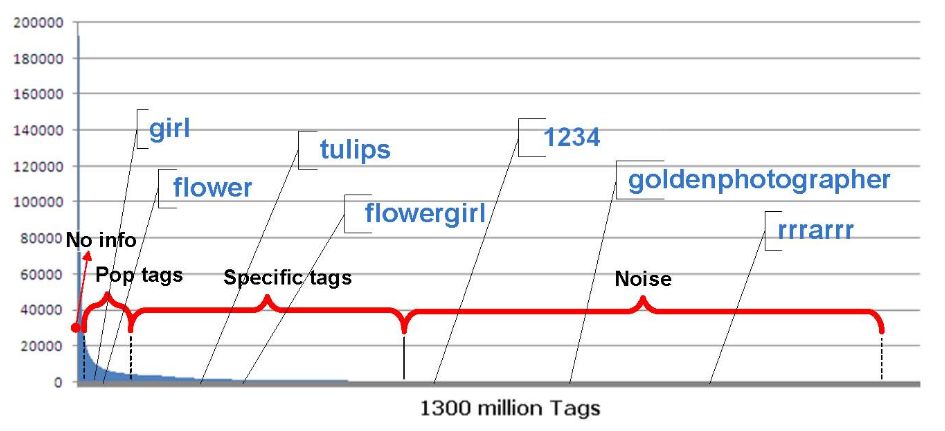
\includegraphics[width=.80\linewidth]{images/fig1.png}
	\end{center}
    Seuls les tags apparaissant entre 50 et 20000 fois dans la base des images étudiées sont pris en compte.

    Le choix de ces deux bornes semble totalement arbitraire car les auteurs ne le justifient à aucun moment.

\end{frame}

\begin{frame}{Critique du protocole de tests}
	
	%
	\begin{itemize}
	\item Les protocoles de tests s'appuient sur un étiquetage humain pour évaluer la couverture des différents modèles. La pertinence d'un tag associé à une image est subjective. Rien n'est dit quand à la redondance de ces évaluations
	\item Le protocole de test décrit la façon de calculer la couverture mais ne dit pas à quoi correspond la précision ni comment elle est calculée
	\item Les auteurs présentent les modèles symétriques et asymétriques mais au final, ils n'indiquent pas clairement quel modèle est utilisé dans les expériences
	\end{itemize}

\end{frame}

\begin{frame}{Problèmes non soulevés}
	
	%
	\begin{center}
        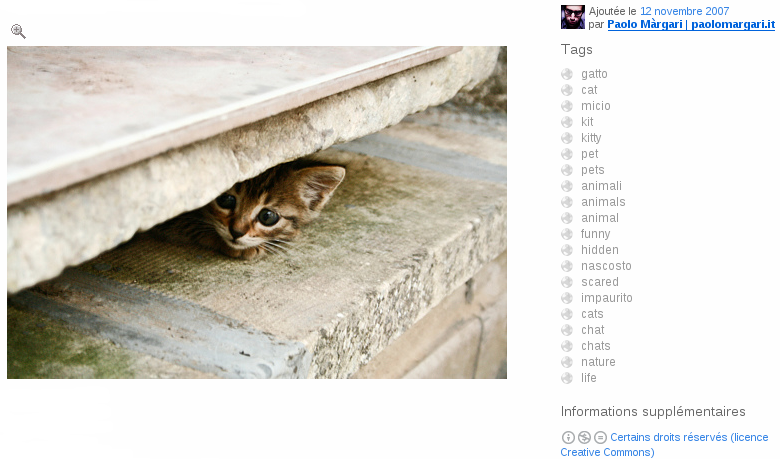
\includegraphics[width=.70\linewidth]{images/capture.png}
	\end{center}
	\begin{itemize}
	\item Une image peut être décrite par des mots de différentes langues
	\item Le mélange des langues risque de poser un problème avec le modèle proposé par les auteurs et ce problème n'est traité à aucun moment
	\end{itemize}

\end{frame}

% End %%%%%%%%%%%%%%%%%%%%%%%%%%%%%%%%%%%%%%%%%

\appendix

\begin{frame}{Fin de la présentation}
	\begin{center}
        Vos questions !
	\end{center}
\end{frame}

\end{document}
